\documentclass{beamer}
\usetheme{Boadilla}
% Choose how your presentation looks.
%
% For more themes, color themes and font themes, see:
% http://deic.uab.es/~iblanes/beamer_gallery/index_by_theme.html
%

%{
%  \usetheme{default}      % or try Darmstadt, Madrid, Warsaw, ...
%  \usecolortheme{default} % or try albatross, beaver, crane, ...
%  \usefonttheme{default}  % or try serif, structurebold, ...
%  \setbeamertemplate{navigation symbols}{}
%  \setbeamertemplate{caption}[numbered]
%}
%\mode<presentation>


\usepackage[italian]{babel}
\usepackage[utf8]{inputenc}
\usepackage[T1]{fontenc}

\title{Rivelatore al Germanio: HPGe}
\author[Pizzati e Virzì]{G. Pizzati. L. Virzì}

\institute[Bicocca]{Università degli Studi di Milano Bicocca}
\date{11 Giugno 2020}

\begin{document}

\begin{frame}
  \titlepage
  \begin{figure}
      \centering
      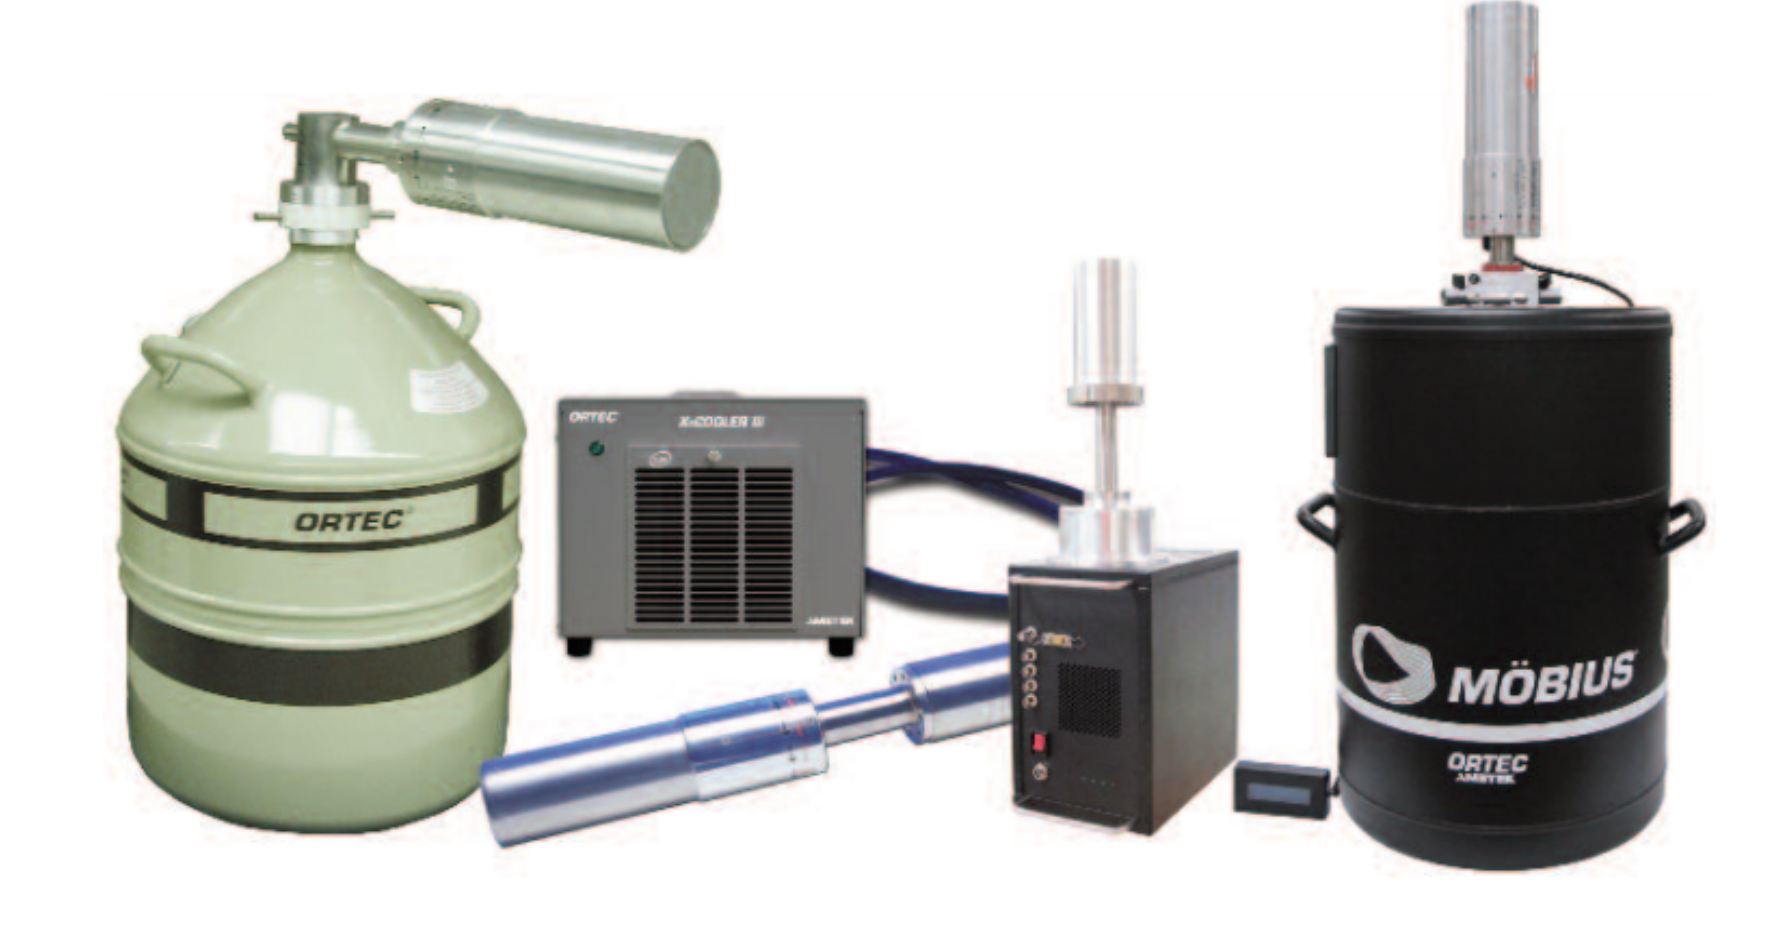
\includegraphics[width=0.4\textwidth]{images/copertina.png}
  \end{figure}
\end{frame}


\begin{frame}{Indice}
  \tableofcontents
\end{frame}

\section{Introduzione Teorica}

\subsection{Funzionamento generale di un rivelatore}
%energia rilasciata da una particella in generale viene assorbita dal rivelatore e convertita in coppie di cariche libere(Bethe-Bloch o Brehmstrahlung o tipi di trasferimento energia dell'fotone). 
\begin{frame}{Funzionamento generale di un rivelatore}
    Un rivelatore è uno strumento che permette l'identificazione di una radiazione a esso incidente, tramito lo studio della corrente $I(t)$ che fluisce al suo interno, e che sorge in seguito all'interazione con la particelle di interesse.
    \begin{itemize}
        \item Scintillazione/Ionizzazione $\to$ cariche libere Q $\to$ segnale elettrico base;
        \item Raccolta cariche dovuta a $\overrightarrow{E}$
        \item Tempo di raccolta: mobilità cariche nel volume attivo, distanza da percorrere, $|E|$
        \item L'arrivo di ogni radiazione è un fenomeno Poissoniano
        \item Ogni interazione produce una corrente univoca e distinguibile
    \end{itemize}
    \begin{equation*}
        \int_{0}^{t_{\textrm{r}}}{I(t)} = Q
    \end{equation*}
\end{frame}

\begin{frame}{Rivelatore - Modalità operative}
    \begin{figure}
        \centering
        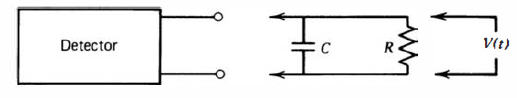
\includegraphics[width=8cm]{images/pulse_mode.png}
    \end{figure}
    Per misure spettroscopiche $\to$ Pulse Mode:
    \begin{itemize}
        \item Circuito di lettura RC;
        \item Integra la corrente su C per ricavare Q, quindi l'energia depositata
        \item Il segnale elettrico di base è la ddp ai capi del carico R
        \item L'ampiezza di un segnale è proporzionale alla carica creata nell'interazione
        \item Preserva le informazioni sui singoli eventi (ampiezza e timing)
    \end{itemize}
    \begin{equation*}
        V_{max} \sim \frac{Q}{C} \sim E
    \end{equation*}
\end{frame}

\subsection{Semiconduttori}
%qui potremmo parlare dei semiconduttori fornendo qualche informazione di base e chiaramente cose attinenti al rivelatore al Germanio(ad esempio in un classico rivelatore a gas ci sono coppie ione-elettrone e l'energia media di produzione è di 25 eV(Argon) mentre qui abbiamo la produzione di coppie elettrone lacuna e l'energia media è invece di 2/3 eV). Questo porta ad avere una maggiore risoluzione a scapito dell'efficienza(se avessimo voluto una maggiore efficienza avremmo potuto prediligere la scelta di uno scintillatore ad alto Z come NaI, Z=53).

%\begin{frame}{Semiconduttori}
%Rivelatori allo stato solido:
%\begin{itemize}
%    \item Maggiore densità rispetto ai rivelatori a gas $\to$ più compatti
%    \item Scintillatori o diodi a semiconduttori. 
%    \item Scintillatori: risoluzione minore (fluttuazioni statistiche nella produzione di portatori di carica), $W \sim 100$ eV, $N_{photoel} \sim 10^3$
%    \item Semiconduttori: $N_{e-h} \sim 10^6$, $W \sim 2-3$ eV
%\end{itemize}
%\medskip
%    Solidi: reticolo cristallino con bande energetiche $\to$ proprietà elettriche
%    \begin{itemize}
%        \item Isolanti, non conducono corrente (gap $\sim 5$ eV);
%        \item Metalli, conducono corrente a qualunque T (no gap);
%        \item Semiconduttori: dipende dalla T e dal drogaggio (gap $\sim 1$ eV).
%    \end{itemize}
%\end{frame}
%usare tanto le bullet list
%\begin{itemize}
%  \item Your introduction goes here!
%  \item Use \texttt{itemize} to organize your main points.
%\end{itemize}

%come fare un blocco evidenziato e centrato
%\vskip 1cm
%\begin{block}{Examples}
%Some examples of commonly used commands and features are included, to help you get started.
%\end{block}

\begin{frame}{Semiconduttori - Struttura a bande}
    Solidi: reticolo cristallino con bande energetiche $\to$ proprietà elettriche
    \begin{itemize}
        \item Isolanti, non conducono corrente (gap $\sim 5$ eV);
        \item Metalli, conducono corrente a qualunque T (no gap);
        \item Semiconduttori: dipende dalla T e dal drogaggio (gap $\sim 1$ eV).
    \end{itemize}
    \begin{figure}
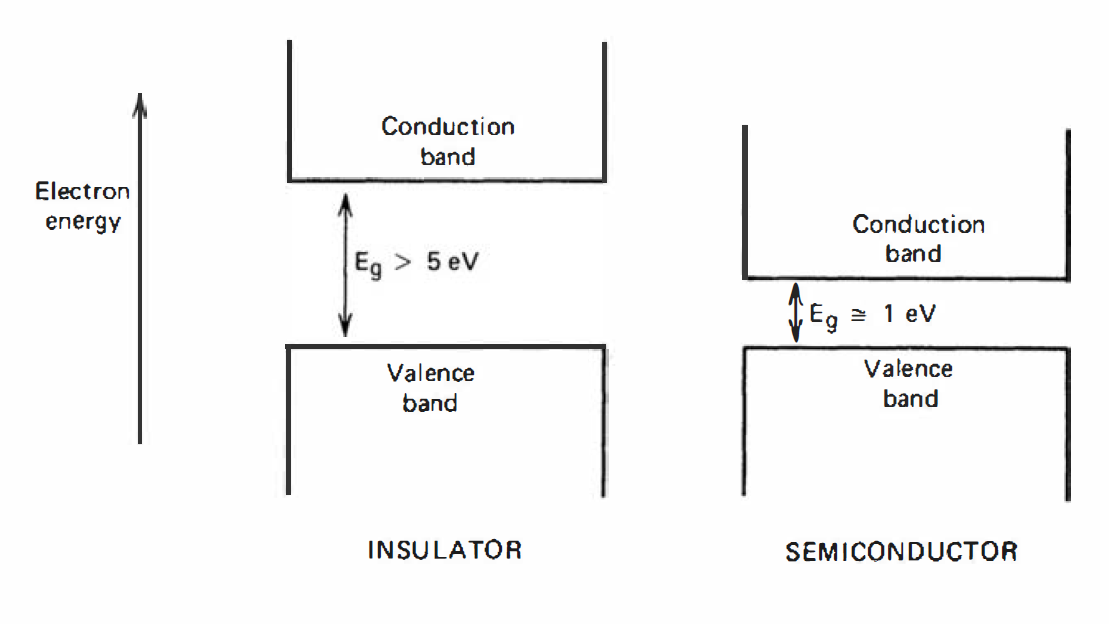
\includegraphics[width=8cm]{images/bandgap.PNG}
\end{figure}
Le bande completamente piene e le bande vuote \textbf{non} conducono corrente!
\end{frame}

%\begin{frame}{Semiconduttori - Portatori di carica}
%    Per T > 0K, gli elettroni del cristallo hanno energia termica.
%    \begin{itemize}
%        \item per $E_{gap}$ piccoli e $T$ alte $\to$ \textbf{elettrone} salta da BV a BC;
%        \item si forma una \textbf{lacuna} nella BV;
%        \item con un $\overrightarrow{E}$ esterno si muovono e contribuiscono alla conduttività, altrimenti si ricombinano nel mezzo.
%    \end{itemize}
%Moto delle cariche:
%\begin{itemize}
%    \item eccitazione termica + velocità data da $\overrightarrow{E}$;
%    \item $e^-$ si muovono in verso opposto al campo, $h^+$ concordi
%    \item velocità inizialmente cresce $\sim E$, poi indipendente (velocità di saturazione, $\sim 10^7$ cm/s)
%    \item $v_{e^-} \sim 2-3\, v_{h^+} \to$ tempi di raccolta simili $\to$ entrambe le correnti vanno integrate per formare un %segnale fedele all'energia incidente
%\end{itemize}
%\end{frame}

\begin{frame}{Semiconduttori intrinseci}
    I principali semiconduttori sono il Silicio e Germanio, elementi del IV gruppo $\to$ 4 legami covalenti coi primi vicini (reticolo a Diamante).
    \begin{itemize}
        \item Occupazione dei livelli alla Fermi-Dirac
        \item Per T = 0 K non conducono corrente, hanno resistività alta
        \item T > 0K, l'agitazione termica crea coppie $e^- h^+$ in ugual numero (ogni elettrone lascia una lacuna nella BV, spostandosi nella BC).  
        \item con un $\overrightarrow{E}$ esterno si muovono e contribuiscono alla conduttività, altrimenti si ricombinano nel mezzo, e all'equilibrio:
        \begin{equation*}
            n_i = p_i
        \end{equation*}
        \item Sono difficili da realizzare
    \end{itemize}
\end{frame}

% SLIDE SOSTITUTIVA PER RIASSUMERE QUELLE SEGUENTI

\begin{frame}{Semiconduttori drogati}
        Le proprietà elettriche dei semiconduttori possono essere migliorate tramite l'aggiunta di atomi di impurezze nel reticolo cristallino.
        \\ Semiconduttori di tipo n:
\begin{itemize}
    \item Drogante del V gruppo (es. Fosforo) $\to$ \textbf{drogaggio n (DONORI).}
    \item Elettroni nella BC dominati dal contributo dei donori ($n = N_D$)
    \item $e^-$ = portatori \textbf{maggioritari}, $h^+$ = portatori \textbf{minoritari}
    \end{itemize}
    Semiconduttori di tipo p:
    \begin{itemize}
    \item Drogante del III gruppo (es. Boro) $\to$ \textbf{drogaggio p (ACCETTORI).}
    \item Si creano delle lacune nella BV senza aumentare gli elettroni nella BC ($p = N_A)$ 
    \item $h^+$ = portatori \textbf{maggioritari}, $e^-$ = portatori \textbf{minoritari}
    \end{itemize}
    Aumentano il numero complessivo di portatori di carica, infatti all'equilibrio:  $n_i p_i = n p$
\end{frame}

%\begin{frame}{Semiconduttori drogati - Semiconduttori di tipo n}
%    Le proprietà elettriche dei semiconduttori possono essere migliorate tramite l'aggiunta di atomi di impurezze nel reticolo %cristallino.
%\begin{itemize}
%    \item Drogante del V gruppo (es. Fosforo) $\to$ \textbf{drogaggio n (DONORI).}
%    \item Occupa un sito del cristallo, ma ha 5 elettroni di valenza $\to$ ne avanza uno debolmente legato.
%    \item Basta poco per eccitarlo alla banda di conduzione, senza lasciare una lacuna nella BV.
%    \item Gli elettroni dei donori occupano un livello interno all'energy gap, vicino alla BC.
%    \item Elettroni nella BC dominati dal contributo dei donori ($n = N_D$)
%    \item Cambia l'equilibrio: $n_i p_i = n p$, ma $n \gg n_i$ $\to$ aumentano i portatori di carica, quindi la conduttività!
%\end{itemize}
%\medskip
%$e^-$ = portatori \textbf{maggioritari}, $h^+$ = portatori \textbf{minoritari}
%\end{frame}

\begin{frame}{Semiconduttori di tipo n}
 La distribuzione di carica rimane complessivamente neutra grazie agli ioni positivi dei donori, fissi. Bilanciano l'eccesso di carica negativa degli elettroni.
          \begin{figure}
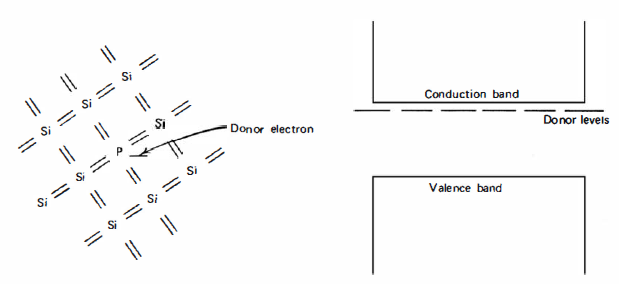
\includegraphics[width=\textwidth]{images/drogaggion.PNG}
\end{figure}  
\end{frame}

%\begin{frame}{Semiconduttori drogati - Semiconduttori di tipo p}
%\begin{itemize}
%    \item Drogante del III gruppo (es. Boro) $\to$ \textbf{drogaggio p (ACCETTORI).}
%    \item Occupa un sito del cristallo, ma ha 3 elettroni di valenza $\to$ avanza una lacuna, simile a quelle lasciate nella BV dagli elettroni che vengono eccitati alla BC.
%    \item Se un elettrone occupa questa lacuna forma un legame covalente, più debole rispetto a quelli del cristallo puro.
%    \item Le lacune degli accettori occupano un livello interno all'energy gap, vicino alla BV. L'eccitazione termica basta a promuovervi gli elettroni.
%    \item Si creano delle lacune nella BV senza aumentare gli elettroni nella BC ($p = N_A)$ 
%    \item Cambia l'equilibrio: $n_i p_i = n p$, ma $p \gg p_i$ $\to$ aumentano i portatori di carica, quindi la conduttività!
%\end{itemize}
%\medskip
%$h^+$ = portatori \textbf{maggioritari}, $e^-$ = portatori \textbf{minoritari}
%\end{frame}

\begin{frame}{Semiconduttori di tipo p}
 La distribuzione di carica rimane complessivamente neutra grazie agli ioni negativi degli accettori, fissi. Bilanciano l'eccesso di carica positiva delle lacune.
          \begin{figure}
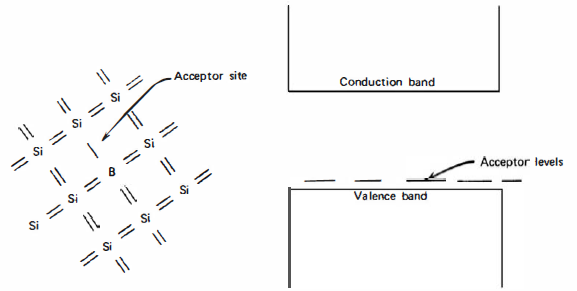
\includegraphics[width=\textwidth]{images/drogaggio_p.PNG}
\end{figure}  
\end{frame}

\begin{frame}{Semiconduttori - Energia di Ionizzazione}
   L'energia di ionizzazione è l’energia media richiesta per la produzione di una coppia di cariche.
   \begin{itemize}
       \item In prima approssimazione, è indipendente dall'energia della radiazione incidente.
       \item Radiazione incidente $\to$ ugual numero di $e^-$ e $h^+$, indipendentemente dal tipo di semiconduttore.
       \item L'energia di ionizzazione piuttosto bassa: $\sim 3$ eV (contro i 30 eV delle camere a ionizzazione).
       \item Numero di cariche prodotto molto alto $\to$ minori fluttuazioni statistiche sul numero di portatori creati $\to$ miglior Signal to Noise Ratio
       \item Formazione del segnale: integro entrambe le correnti
   \end{itemize}
\end{frame}

\begin{frame}{Rivelatori a semiconduttore - Giunzione pn}
Una \textbf{giunzione pn} consiste nel drogaggio di due regioni del cristallo con impurità di tipo p e n, poste in contatto termodinamico tra di loro. Alle estremità delle regioni p e n vengono collegati due contatti metallici (p $\to$ anodo, n $\to$ catodo).
    \begin{itemize}
        \item Discontinuità nella densità di $e^-$ alla giunzione $\to$ gradiente $\to$ \textbf{corrente di diffusione} delle cariche.
        \item $e^-$: regione \textbf{n} $\to$ regione \textbf{p}, dove si ricombinano con le lacune.
        \item La diffusione degli $e^-$ porta alla formazione di ioni + immobili nella regione \textbf{n}.
        \item Le lacune $h^+$ seguono il percorso inverso.
    \end{itemize}
    \medskip
    Risultato: si creano due regioni con carica spaziale fissa positiva (lato n) e negativa (lato p) ai lati della giunzione. Diminuiscono le cariche libere in prossimità della giunzione (\textbf{regione svuotata}). Si creano quindi un campo elettrico e una ddp che si oppongono alla diffusione.
\end{frame}

\begin{frame}{Rivelatori a semiconduttore - Giunzione pn}
    \begin{figure}
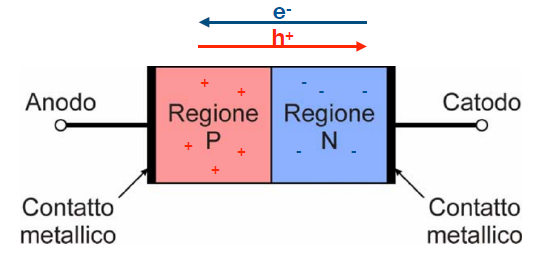
\includegraphics[width=6cm]{images/giunzione_pn_1.PNG}
\end{figure}  
\begin{figure}
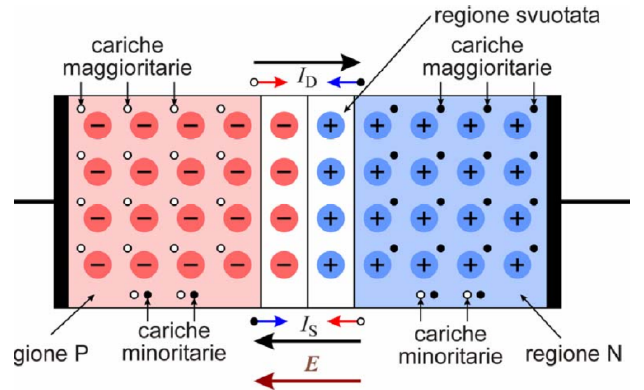
\includegraphics[width=6cm]{images/giunzione_pn_2.PNG}
\end{figure}  
\end{frame}

\begin{frame}{Rivelatori a semiconduttore - Regione di svuotamento}
    Ha delle ottime caratteristiche per il rilevamento di radiazioni:
    \begin{itemize}
        \item Cariche fisse (ioni) $\to$ alta resistività;
        \item La barriera di potenziale ed $\overrightarrow{E}$ ostacolano il moto delle cariche \textbf{maggioritarie} $\to$ $e^-$ verso la regione p e $h^+$ verso la regione n (corrente di diffusione $I_D$);
        \item Se una radiazione incidente genera delle coppie in questa regione, vengono portate fuori (moto di cariche $\to$ corrente che costituisce il segnale);
        \item Continua la produzione di cariche minoritarie per \textbf{eccitazione termica}, il cui passaggio è favorito dal campo $\overrightarrow{E}$ \\ (\textbf{corrente di deriva $I_S$}).
    \end{itemize}
    All'equilibrio non scorre corrente nella giunzione, poiché vale:
    \begin{equation*}
        I_S = I_D
    \end{equation*}
\end{frame}

\begin{frame}{Rivelatori a semiconduttore - Polarizzazione inversa}
    Senza una tensione esterna, il rivelatore avrebbe una risoluzione piuttosto bassa.  La $V_0$ ai capi della giunzione è bassa ($\sim 1$ V), e i portatori di carica sono lenti $\to$ ricombinazione e raccolta incompleta. 
    \\ Viene quindi applicata una tensione esterna $V_{bias}$:
    \begin{itemize}
        \item \textbf{Polarizzazione inversa} $V$ all'anodo (p) < $V$ al catodo (n)
        \item Una polarizzazione diretta facilita il passaggio delle cariche maggioritarie ($I_D)$, quella inversa lo ostacola ($\sim$ diodo).
        \item Le cariche \textbf{minoritarie} sono attratte attraverso la giunzione ($I_S$).
        \item La concentrazione dei minoritari è piccola, e la loro corrente dipende sostanzialmente da $T$ ed $E_{gap}$.
    \end{itemize}
    \medskip
    Vale infatti:
    \begin{equation*}
        I_{fuga} \sim T^{\frac{3}{2}}\,e^{-\frac{E_g}{kT}}
    \end{equation*}
\end{frame}

\begin{frame}{Polarizzazione inversa}
\begin{itemize}
    \item Rafforza $V_0$ ai capi della regione;
    \item Si allarga la regione svuotata $\to$ aumenta il volume attivo (full o over depleted).
    \item Radiazione incidente deposita energia nella regione di svuotamento e genera coppie $e^-h^+$, che si muovono sotto l'azione di $V_{bias}$ $\to$ $I_{segnale}$
    \item $I_{segnale}$ si sovrappone a $I_S$ dei minoritari, che aumenta con l'allargarsi del volume attivo $\to$ sfalsa il segnale $\to$ bagno criostatico (Ge @ 77 K) 
\end{itemize}
    Valgono le relazioni:
    \begin{equation*}
        d \simeq \sqrt{\frac{2\varepsilon V}{eN}} \,\,\,\,\,\,\,\,\,\,\,\,\,C = \frac{\varepsilon S}{d} \sim \frac{1}{\sqrt{V}}
    \end{equation*}
    con $V$ = $V_{bias}$, $\varepsilon$ costante dielettrica del mezzo e $N$ concentrazione del drogante predominante.
    \\ Per avere $d$ grande e $C$ piccola $\to$ basse $N$ e $V$ alte $\to$ HPGe!
\end{frame}

%
%\subsection{Funzionamento generale di un rivelatore}
%energia rilasciata da una particella in generale viene assorbita dal rivelatore e convertita in coppie di cariche libere(Bethe-Bloch o Brehmstrahlung o tipi di trasferimento energia dell'fotone). 
%\begin{frame}{Funzionamento generale di un rivelatore}
%    
%\end{frame}

\begin{frame}{Rivelatori per raggi Gamma}
    \begin{itemize}
        \item Fotone con energia tra circa 100 keV e 2615 keV(per catene di decadimento naturali), ma è una particella neutra, quindi no Bethe Bloch
        \item Effetto Fotoelettrico $\to$ Fotopicco
        \item Scattering Compton $\to$ Continuo e Spalla Compton
        \begin{equation}
            E'_{\textrm{fotone}} = \frac{E}{1+\frac{E}{m_e c^2} (1-cos\theta)}
        \end{equation}
        \item Produzione di coppia($e^-e^+$) $\to$ Positronio $\to$ Possibile fuoriuscita di uno o due gamma
    \end{itemize}
    \begin{figure}
        \centering
        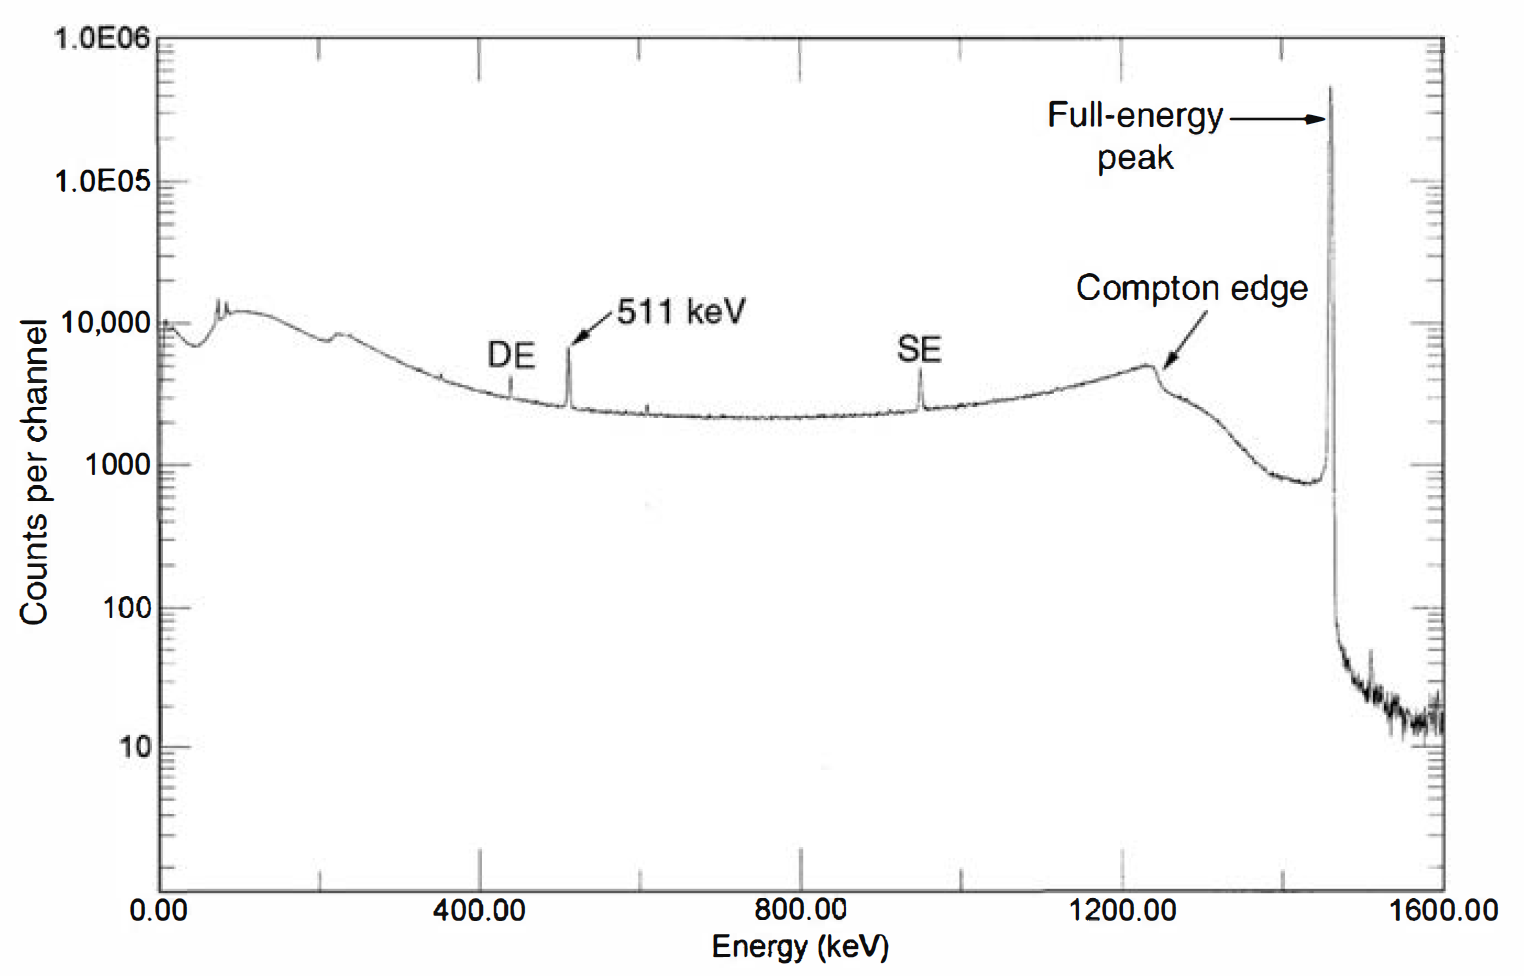
\includegraphics[width=0.4\textwidth]{images/spettro_gamma.png}
        \label{fig:my_label}
    \end{figure}
\end{frame}

\section{HPGe}


\subsection{Principi}
%introduzione con le figure all'HPGe
\begin{frame}{Rivelatori a semiconduttore - HPGe}
    \begin{itemize}
        \item Adatto alla spettroscopia $\gamma$, ottima risoluzione
        \item Germanio High Purity: impurità $\sim 10^9-10^{10}$ atomi/cm$^3$
        \item Regione di svuotamento di alcuni cm ($V_{bias} \sim 3-5$ kV, poi ho breakdown e forti $I_{fuga}$)
        \item Configurazione planare o coassiale
        \item Polarizzazione inversa alla giunzione pn: voltaggio positivo su n$^+$, negativo su p$^+$
        \item $V_{bias}$ alto: overvoltage (campo uniforme, evita raccolta incompleta)
        \item $E_{gap_{Ge}} = 0.67$ eV $\to$ bagno criostatico (N$_2$, 77 K)
            \end{itemize}
        \begin{minipage}{\linewidth}
      \centering
      \begin{minipage}{0.45\linewidth}
          \begin{figure}[H]
              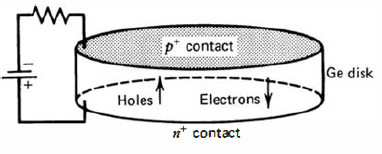
\includegraphics[width=\linewidth]{images/planare.PNG}
          \end{figure}
      \end{minipage}
      \hspace{0.05\linewidth}
      \begin{minipage}{0.45\linewidth}
          \begin{figure}[H]
              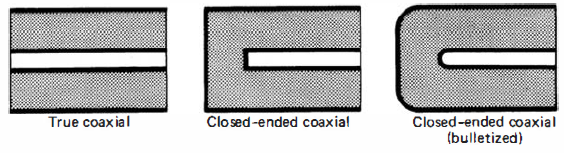
\includegraphics[width=\linewidth]{images/coaxial.PNG}
          \end{figure}
      \end{minipage}
  \end{minipage}
 
\end{frame}

\begin{frame}{HPGe Coaxial}
\begin{itemize}
    \item Impurità residue di tipo p: HPGe-$\pi$ type (altrimenti $\nu$ type)
    \item Volume attivo molto grande (800 cm$^3$ contro i 10 dei planari)
    \item Raggio interno piccolo $\to$ capacità bassa $\to$ risoluzione maggiore
    \item I contatti elettrici formano le \textbf{giunzioni pn} (Reverse Bias)
    \item Contatto esterno $\to$ raddrizzatore (necessita di $V_{bias}$ minore)
    \item Terminali elettrici sottili: passano radiazioni poco penetranti e diminuisce lo strato morto (attenuazione minima)
    \item Adatti a spettroscopia su ampio range di energie (keV $\div$ MeV)
\end{itemize}
    \begin{figure}
        \centering
        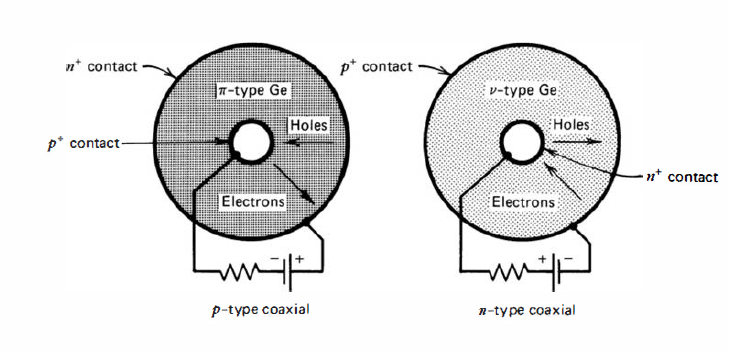
\includegraphics[width=8cm]{images/hpge_coaxial.PNG}
    \end{figure}
\end{frame}

\begin{frame}{HPGe - Condizioni operative}
\begin{itemize}
    \item Moderni HPGe: raffreddati solo durante l'uso
    \item Reservoir a 77 K + Camera a vuoto (alternative: He/refrig. meccanica $\to$ vibrazioni!)
    \item Le performance iniziano a peggiorare attorno ai 130 K
    \item Il vuoto inibisce la conduttività termica tra il cristallo e l'aria circostante, ed evita la condensazione di vapori $\to$ contaminazioni che peggiorano la risoluzione e rovinano il rivelatore
    \item Evita la dispersione di carica quando $V_{bias}$ è alta
    \item Obiettivo: ridurre il rumore di fondo (schermi metallici)
    \item HPGe moderni: preamplificatore inglobato nel criostato
 \end{itemize}
    
\end{frame}

\subsection{Risoluzione HPGe}
   
\begin{frame}{Risoluzione degli HPGe}
\begin{itemize}
    \item Spettroscopia di radiazione $\to$ quanto sono piccati i picchi?
    \item Definisco Risoluzione in funzione della FWHM
     \begin{figure}
        \centering
        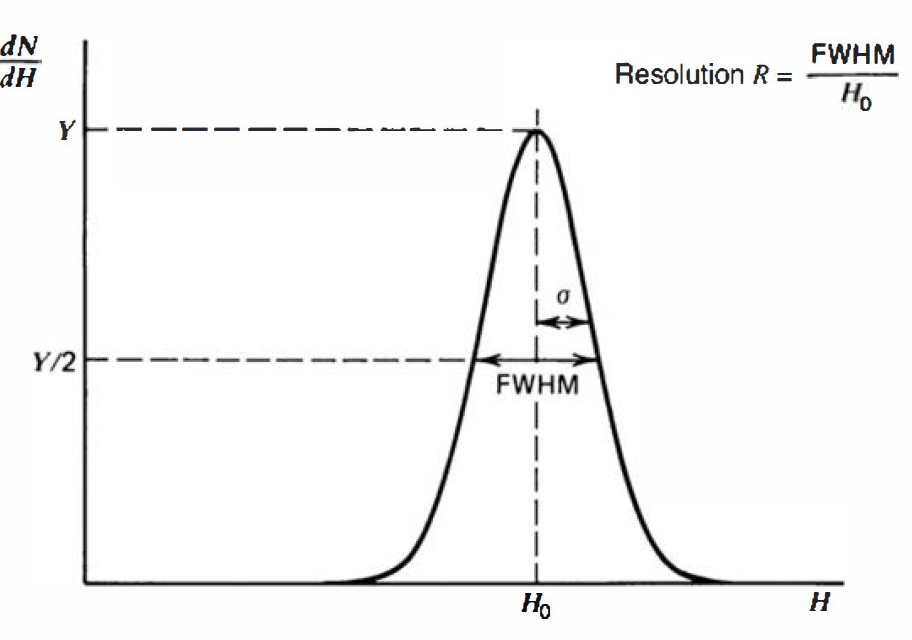
\includegraphics[width=0.5\textwidth]{images/fwhm_resolution.png}
    \end{figure}
    \item È una quantità adimensionale e spesso riportata in percentuale $\to$ per HPGE a 1332 keV è 0.14\% 
   \item Ci dice quanto possiamo distinguere due picchi vicini
    \end{itemize}
    
\end{frame}
\begin{frame}{Risoluzione degli HPGe continua...}
\begin{itemize}
    \item Approx. Poissoniana: fluttuazione nella produzione di $N$ coppie è $\sqrt{N}$ $\to$ se N grande allora picco è Gaussiana $\to$  $R=\frac{2.35 \sigma}{H_0}$
    \item In realtà non è proprio Poissoniana(per fortuna) $\to$ introduco il fattore di Fano: \begin{equation}
        \frac{\textrm{varianza misurata su N}}{\textrm{varianza di Poisson(=N)}}
    \end{equation}
    \item Quindi risoluzione diventa:\begin{equation}
        R = \frac{2.35 K \sqrt{N} \sqrt{F}}{K N} = 2.35 \sqrt{\frac{F}{N}}
    \end{equation}
    
    \item Diversi fattori determinano allargamento(non solo statistica portatori carica): \begin{equation}
        (FWHM)^2_{tot} = (FWHM)^2_{stat} + (FWHM)^2_{elettr.} + (FWHM)^2_{racc.inc.} 
    \end{equation}
    \item Perché risoluzione HPGe è tanto buona?\begin{enumerate}
        \item Fano basso(0.08-0.15) e bassa $\omega = 2.96$ eV
        \item Detector piccolo e campi elettrici intensi(tanto da saturare velocità portatori carica)
    \end{enumerate}
\end{itemize}
    
    
        
\end{frame}

\subsection{Pulse Shape e Spettroscopia gamma con HPGe}
\begin{frame}{Processo raccolta cariche}
\begin{itemize}
    \item Shaping time elettronica dedicata a formazione segnale > rise-time del segnale rivelatore(per PHA e quindi spettroscopia)
    \item Informazione sul timing da rise-time e dalla forma del fronte di salita
    \item Fronte di salita determinato da caratteristiche processo di raccolta della carica
    \item Visto che si vogliono rise time sempre più piccoli $\to$ bisogna avere raccolta cariche molto veloce $\to$ campi molto intensi $\to$ velocità portatori di carica satura alla velocità di deriva($\sim 10^5$ m/s)
    \item Limiti: \begin{enumerate}
        \item tempi raccolta ordine 100 ns(per detector piccoli)
        \item forma segnale dipende da dove interagisce particella $\to$ fronte assumerà forme che variano
    \end{enumerate} 
\end{itemize}
    
\end{frame}

\begin{frame}{Spettroscopia gamma con HPGe}
    \begin{itemize}
        \item Abbiamo buona risoluzione(0.14\% a 1332 keV contro 5-10\% NaI) ma un cattiva efficienza nel fotopicco(causa basso Z e piccole dimensioni)
        \item Buona risoluzione permette distinguere non solo picchi vicini ma anche picchi poco intensi perché molto piccati e "spiccano" sul fondo
        \item Scelta HPGe ottima per spettri gamma complessi, mentre NaI meglio se ci sono pochi picchi e poco intensi
    \end{itemize}
    \begin{figure}
        \centering
        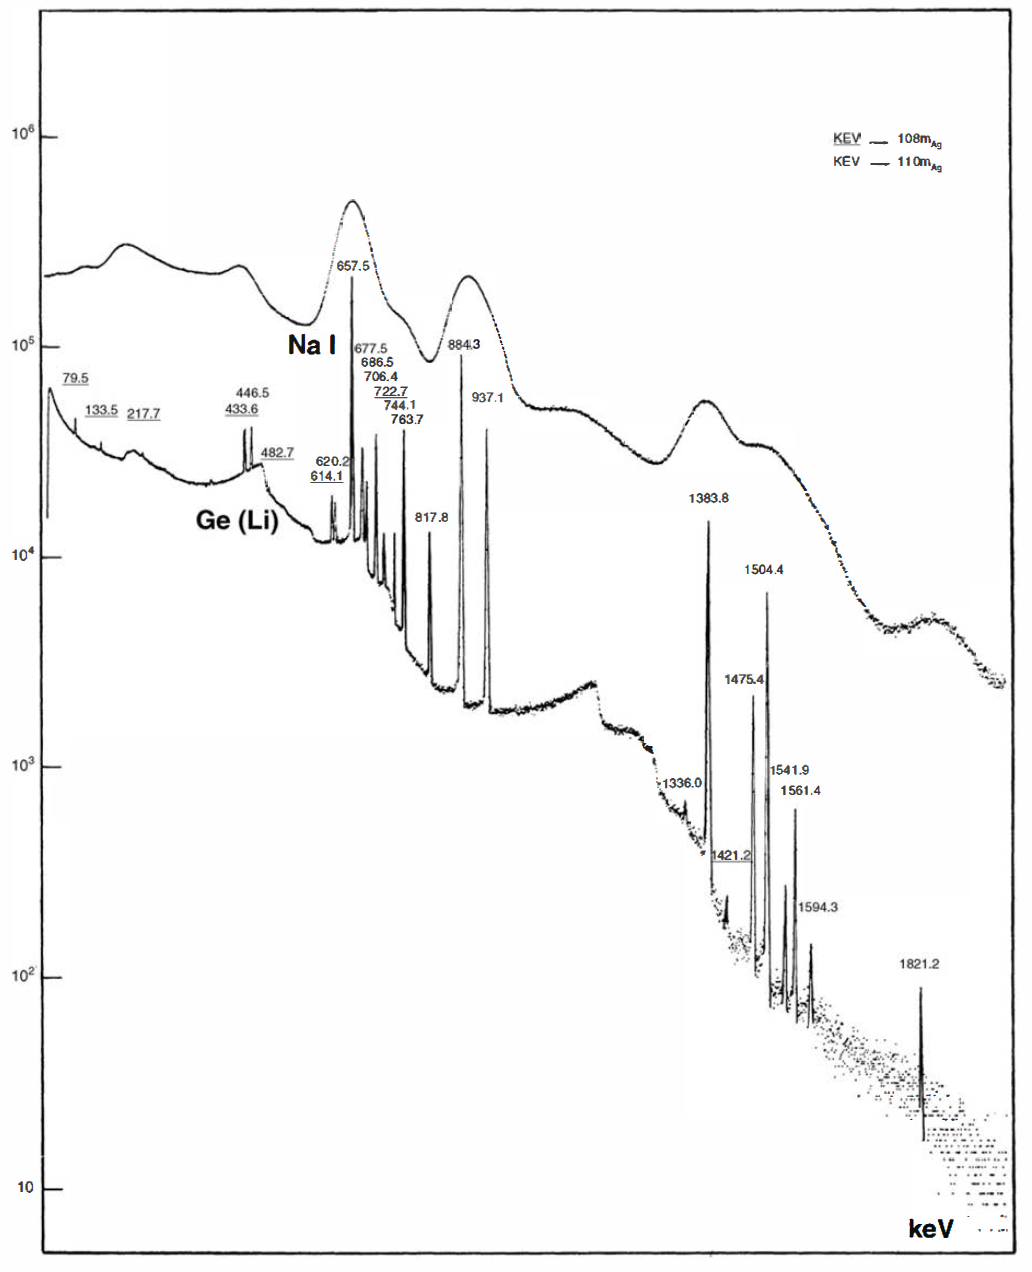
\includegraphics[width=0.3\textwidth]{images/confronto_spettro_hpge_nai.png}
    \end{figure}
\end{frame}

\begin{frame}{Funzione di risposta}
    \begin{itemize}
        \item Il continuo Compton è accentuato in questi rivelatori(rispetto ad NaI) quindi più eventi ma spalla Compton sempre nella stessa posizione
        \item Essendo un piccolo rivelatore e a basso Z sarà più probabile fuoriuscita radiazione $\to$ escape peaks(sia degli X sia relativi a positronio)
        \item Produzione di coppia con Single e Double Escape Peak
        \item Inoltre si ha allargamento picco a 511 keV causato da momento non nullo del positronio $\to$ 2 gamma prodotti in volo $\to$ Effetto Doppler $\to$ Allargamento picco
        \item Forma del picco $\to$ Presenza Coda $\to$  Full Width at One-Tenth Maximum(FW0.1M)
    \end{itemize} 
\end{frame}

\subsection{Efficienza HPGe}
%arriva fino a 150% se paragonata a NaI...
\begin{frame}{HPGe - Efficienza}
    In letteratura vengono riportati diversi tipi di efficienza (totale, FE-peak, DE, SE), e ognuna può essere:
    \begin{itemize}
        \item Intrinseca = probabilità che un $\gamma$ a $E$ fissata incida sul rivelatore e venga conteggiato (dipende da $E$ e $L$ detector)
        \item Assoluta = probabilità che un $\gamma$ emesso da una specifica sorgente venga conteggiato ($E$, geometria rivelatore, distanza)
        \item Relativa = rapporto tra la rispettiva efficienza assoluta e uno standard preso come riferimento (@1332 keV del $^{60}$Co su un NaI 3'' x 3'' a 25cm)
        \item Effficienza bassa, compensata dalla risoluzione $\to$ picchi alti
        \item Formule empiriche (ma si ricorre a calibrazioni/MC)
        \item Altro parametro d'interesse: \emph{peak-to-Compton Ratio}
    \begin{equation*}
        PCR =  \frac{\textrm{(altezza del picco a 1.33 MeV)}}{\textrm{(altezza media del plateau Compton del picco)}}
    \end{equation*}
     \end{itemize}
\end{frame}


\section{Elettronica di Lettura}
%catena di lettura, preamp, amp, rumore e discussione riprendendo le slides introduttive della schematizzazione del circuito del rivelatore.

\begin{frame}{Schematizzazione base di un detector}
\begin{itemize}
    \item La radiazione incidente rilascia una certa energia producendo coppia di portatori cariche(e-h). 
    \item Le cariche prodotte vengono raccolte grazie alla presenza di un campo elettrico. Le cariche generano una certa corrente i(t) nel rivelatore che viene integrata nel preamp.
    \item Il Pulse Shaping e l'amplificatore formano e amplificano il segnale
    \item L'MCA converte il segnale in un numero digitale e lo memorizza per poi formare il Pulse Height Spectrum
\end{itemize}
\begin{figure}
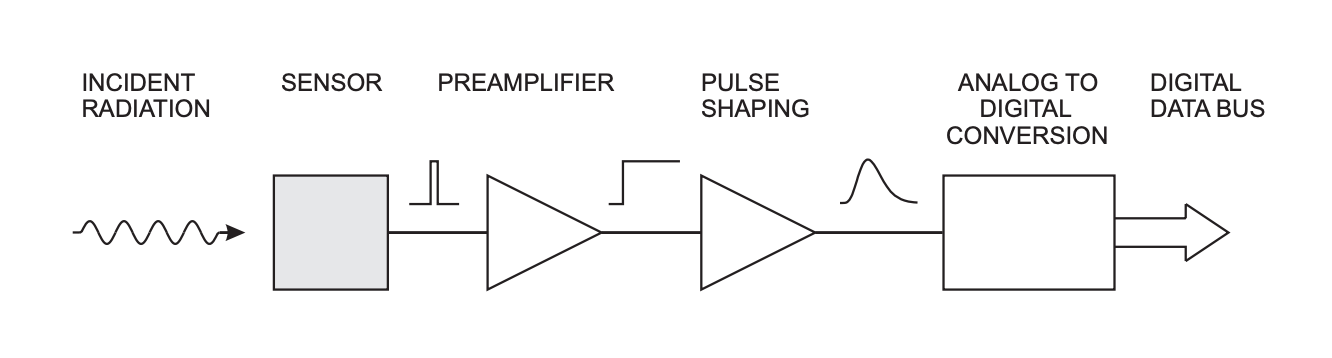
\includegraphics[width=\textwidth]{images/basic_detector_function.png}
\end{figure}


\end{frame}



\subsection{Preamplificatore}
\begin{frame}{Preamplificatore}
Funzionalità Preamp:
\begin{itemize}
    \item Fornire accoppiamento ideale tra segnale detector e catena lettura
    \item Integrare segnale detector $\to$ Configurazione Charge\-Sensitive
    \item \begin{equation}
            V_{out} = -A \frac{Q}{C_{in}+(A+1)C_f} \sim \frac{Q}{C_f}
        \end{equation}
    \item Rise time veloce(ns) e poi decadimento molto lento($\sim 100 \mu s$)
    \item Rumore Preamp
\end{itemize}

    \begin{figure}
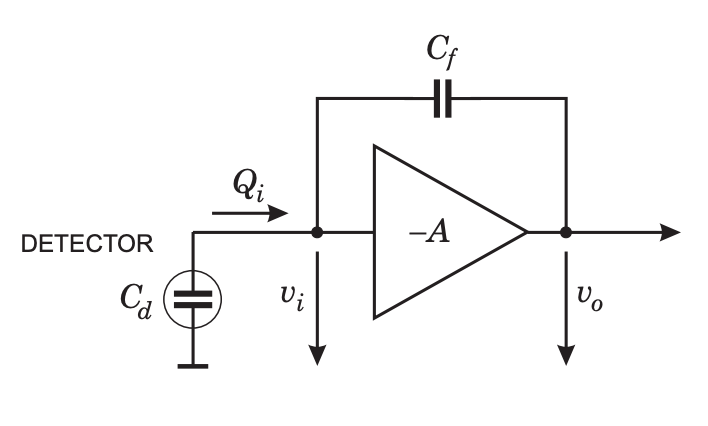
\includegraphics[width=0.4\textwidth]{images/charge_sensitive_amplifier.png}
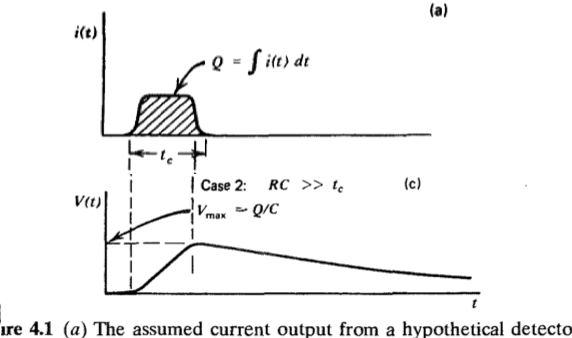
\includegraphics[width=0.4\textwidth]{images/scelta_RC.png}
\end{figure}
\end{frame}


\subsection{Segnale, rumore e Pulse Shaping}


\begin{frame}{Segnale e rumore}
    \begin{itemize}
    \item ENC: Q t.c. S/N = 1
    \item Nota l'ENC $\to$ $FWHM_{el} = 2.35 \cdot 2.96 eV \cdot  ENC $, dove ENC è espressa in unità di $e^-$
    \item $ENC^2(\tau_{shaping}) \sim (\frac{C^2}{\tau}+\tau I)$
    \item Noise vs $V_{bias}$: \begin{enumerate}
        \item $Noise \sim C_d \sim \frac{1}{\sqrt{V}}$ <- rumore serie a bassi $V_{bias}$
        \item $Noise \sim i_{bias} \sim V$
    \end{enumerate}
\end{itemize}
\end{frame}

\begin{frame}{ENC vs Shaping Time}
    \begin{figure}
    \centering
    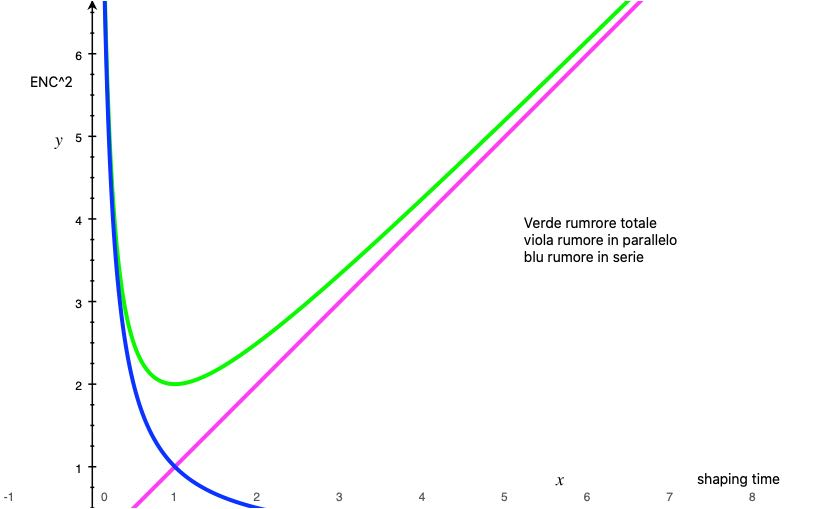
\includegraphics[width=0.8\textwidth]{images/grafico_rumore.jpg}
\end{figure}
\end{frame}

\begin{frame}{Amplificatori e Pulse Shaping}
\begin{itemize}
    \item Pulse Shaping:
    \begin{itemize}
        \item CR$-$RC shaping: CR diff. e RC integr
        \item La combinazione delle due reti permette di arrotondare picco e tagliare la coda $\to$ migliore S/N
        \item Rete disaccoppiata da op. amp. ideale
        \item Si possono mettere tanti RC dopo per avere una forma gaussiana
        \item Obbiettivo P.S.:  \begin{enumerate}
            \item evitare il pile up(tagliando code)
            \item migliorare S/N stringendo B.P.
        \end{enumerate}
        \item Problema è che segnale del preamp. non è un gradino $\to$ undershoot che si rimuove aggiungendo resistenza in $//$ a C del CR con cancellazione di polo zero
    
    \end{itemize}
    \item Amplificatori:
    \begin{itemize}
        \item È il principale stadio di guadagno nella catena di lettura($G \sim 10^3$)
        \item Problema della $V_{bias}$
    \end{itemize}
\end{itemize}
Risp. al gradino CR$-$RC nel caso di $\tau_{CR}=\tau_{RC}$
    \begin{equation}
        V_{out} = V \frac{t}{\tau} e^{-\frac{t}{\tau}}
    \end{equation}
    
\end{frame}

\begin{frame}{ADC/MCA}
    \begin{itemize}
        \item Memorizza altezza segnali in canali
        \item Dai canali si passa allo spettro energetico(perché $V_{max}\sim E_{\textrm{rilasciata}}$)
        \item Idealmente dovrebbe creare retta calibrazione passante per origine $\to$ in realtà offset
        \item Usato anche per misure di tempo con TAC in modalità Multichannel Scaling(si contano eventi in funzione del tempo)
        \item A noi interessa Pulse Height Analysis $\to$ ADC converte altezza segnale in arrivo in numero digitale
        \item Tempo morto dovuto a \begin{enumerate}
            \item Rise time segnale
            \item Tempo di conversione
            \item Tempo memorizzazione
        \end{enumerate}
    \end{itemize}
\end{frame}

\begin{frame}{Applicazione dei rivelatori al Germanio}
    
    \textbf{Large Enriched Germanium Experiment for Neutrinoless $\beta \beta$ decay}
       \begin{columns}
           \begin{column}{0.4\textwidth}
              
\includegraphics[width=2.5cm]{images/gerda.PNG}
           \end{column}
           \begin{column}{0.4\textwidth}
           BroadEnergy Germanium: 
           \begin{itemize}
           \item GERDA 
           \item LEGEND-200
           \end{itemize}
           \end{column}
        \end{columns}
        
    \textbf{Cryogenic Dark Matter Search (CDMS)}
    \begin{figure}
    \centering
    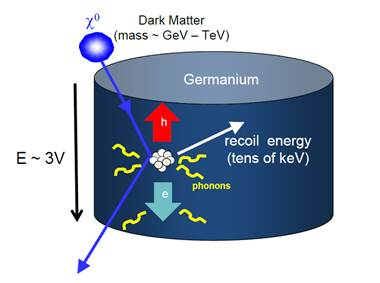
\includegraphics[width=5.6cm]{images/cdms.png}
\end{figure}
    \end{frame}
    
\begin{frame}{Applicazioni dei rivelatori al Germanio}
    \begin{itemize}
        \item Data l'ottima risoluzione usata tutt'ora come rivelatore per misure di radioattività
        \item Diversi studi fatti ai Laboratori di Radioattività di MiB e Low Activity Lab di LNGS
        \item Ad esempio per selezionare materiali con bassissima radioattività(elementi puri fino al ppt e attività dell'ordine dei 10 mBq/kg(MiB) o 100 $\mu$Bq/kg)  o studio radioattività in campioni d'acqua
    \end{itemize}
\end{frame}

\begin{frame}{Fine Presentazione}
    Grazie dell'attenzione e scusate se abbiamo sforato il tempo per la presentazione
    :)
    \vfill
    Giorgio e Luca
    
    
\end{frame}


\end{document}
